\documentclass{article}
\usepackage[utf8]{inputenc}
\usepackage{hyperref}
\usepackage[letterpaper, portrait, margin=1in]{geometry}
\usepackage{enumitem}
\usepackage{amsmath}
\usepackage{booktabs}
\usepackage{graphicx}
\usepackage{longtable}

\usepackage{hyperref}
\hypersetup{
colorlinks=true,
    linkcolor=black,
    filecolor=black,      
    urlcolor=blue,
    citecolor=black,
}
\usepackage{natbib}

\usepackage{titlesec}
  
\title{Homework 2}
\author{Ryan Ellis}
\date{\today}

  
\begin{document}
  
\maketitle

\section{Python}
\subsection{Comparison of means}


\begin{longtable}{llll}
\hline
 Variable       & Mean($D_{1i}$)   & Mean($D_{0i}$)   & Diff.-in-means (p-val)   \\
\hline
\endhead
 Electricity    & 1086.75                 & 1181.33               & 0.001                          \\
                & (423.96)                & (454.31)              &                                \\
 Square Footage & 1657.55                 & 1633.05               & 0.572                          \\
                & (686.27)                & (682.90)              &                                \\
 Retrofit       & 1.00                    & 0.00                  & 0.0                            \\
                & (0.00)                  & (0.00)                &                                \\
 Temperature    & 79.89                   & 79.89                 & 0.987                          \\
                & (1.97)                  & (2.16)                &                                \\
\hline
\end{longtable}


It appears randomization worked here. The home locations (proxied by "Temperature") and sizes ("Square Footage") are similar across treatment and control. The difference in mean outcome, if indeed we have complete random assignment, is the Average Treatment Effect.

\subsection{Kernel Density Plot}

\begin{figure}[ht]
    \centering
    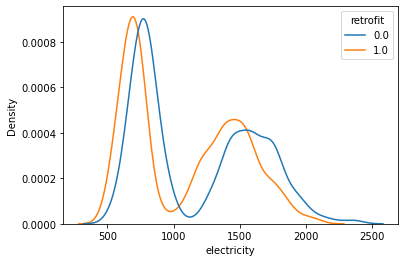
\includegraphics[scale = 0.7]{kdeplot.png}
    \caption{Treated households shown in orange}
\end{figure}

\vspace{5cm}


\subsection{OLS Methods}

\begin{longtable}{lrrr}
\hline
           &     By hand &   Simulation &      Canned \\
\hline
\endhead
 Intercept &  -83.6028   &   -83.611    &  -83.6028   \\
 retrofit  & -109.666    &  -109.666    & -109.666    \\
 sqft      &    0.615339 &     0.615339 &    0.615339 \\
 temp      &    3.25508  &     3.25518  &    3.25508  \\
\hline
\end{longtable}


\section{Stata}

\subsection{Comparison of means}


\begin{table}[ht]
    \centering
    {
\def\sym#1{\ifmmode^{#1}\else\(^{#1}\)\fi}
\begin{tabular}{l*{3}{cccc}}
\hline\hline
            &\multicolumn{4}{c}{(1)}                                     &\multicolumn{4}{c}{(2)}                                     &\multicolumn{4}{c}{(3)}                                     \\
            &\multicolumn{4}{c}{}                                        &\multicolumn{4}{c}{}                                        &\multicolumn{4}{c}{}                                        \\
            &        Mean&   Std. Dev.&     T-stat.         &     p-value&        Mean&   Std. Dev.&     T-stat.         &     p-value&        Mean&   Std. Dev.&     T-stat.         &     p-value\\
\hline
electricity &     1086.75&    (423.96)&                     &            &     1181.33&    (454.31)&                     &            &            &            &      94.584\sym{***}&     (3.404)\\
sqft        &     1657.55&    (686.27)&                     &            &     1633.05&    (682.90)&                     &            &            &            &     -24.499         &    (-0.566)\\
retrofit    &        1.00&      (0.00)&                     &            &        0.00&      (0.00)&                     &            &            &            &      -1.000         &         (.)\\
temp        &       79.89&      (1.97)&                     &            &       79.89&      (2.16)&                     &            &            &            &      -0.002         &    (-0.016)\\
\hline
\(N\)       &         499&            &                     &            &         501&            &                     &            &        1000&            &                     &            \\
\hline\hline
\end{tabular}
}

    \caption{produced using Stata}
    \label{tab:statasummary}
\end{table}


\subsection{Scatter plot}

\begin{figure}[ht]
    \centering
    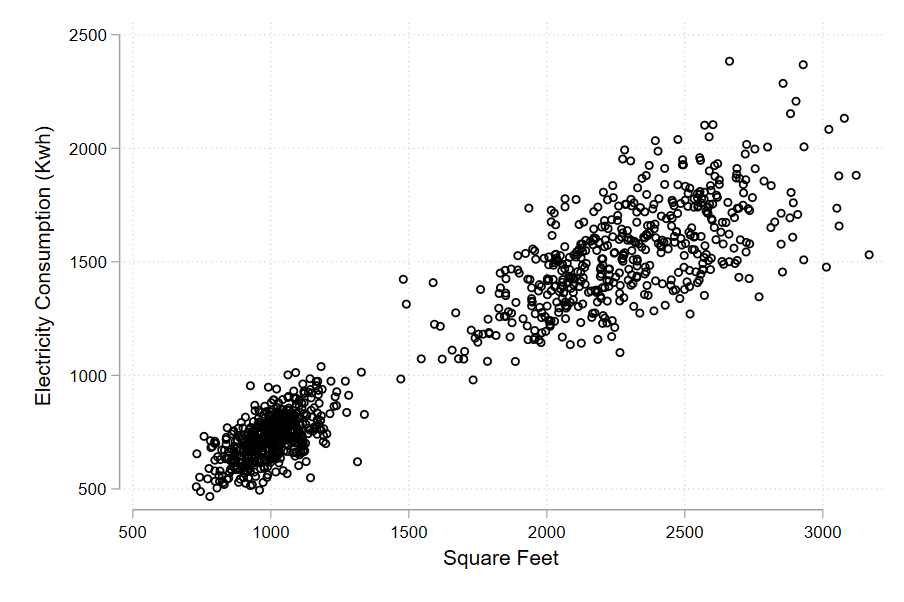
\includegraphics[scale = 0.4]{scatter_stata.png}
    \caption{Scatter plot produced in Stata with \textit{twoway}}
\end{figure}
\vspace{5cm}

\subsection{Regression}

\begin{table}[ht]
    \centering
    \begin{tabular}{lc} \hline
 & (1) \\
VARIABLES & electricity \\ \hline
 &  \\
retrofit & -109.7*** \\
 & (7.943) \\
sqft & 0.615*** \\
 & (0.00678) \\
temp & 3.255* \\
 & (1.932) \\
Constant & -83.60 \\
 & (154.7) \\
 &  \\
Observations & 1,000 \\
 R-squared & 0.919 \\ \hline
\multicolumn{2}{c}{ Robust standard errors in parentheses} \\
\multicolumn{2}{c}{ *** p$<$0.01, ** p$<$0.05, * p$<$0.1} \\
\end{tabular}

    \caption{produced using Stata}
    \label{tab:statasummary}
\end{table}

\end{document}